%!TEX root =  ../samplepaper.tex
\section{Background}
%Proof systems are fundamental in logic education because they provide a structured framework for understanding and constructing logical arguments, ensuring rigor and validity in mathematical reasoning. Among the many proof systems, one usually adopted in the logic courses is the Natural Deduction (ND) system, which was defined to more closely align with mathematical and everyday reasoning under assumptions~\cite{nd-mancosu}. It emerged in 1934 with Gentzen and Jaśkowski's work, gaining widespread acceptance by the 1960s~\cite{Pelletier1999-FRAABH}. In a ND system we can construct proofs showing that a formula \(\varphi\) is a logical consequence of a set of formulas \(\Gamma\), written \(\Gamma \vdash \varphi\). 
%\cmt{O documento Gouveia e Dionisio nao deve ser citado por ser apenas um draft. Já agora, podemos usar este comando para deixar comentários ao longo do texto. Depois é fácil desativar todos de uma só vez.}
There are two main styles of presenting ND proofs. One is the Gentzen-style, which organizes the proof in a tree-shaped structure, also known as deduction tree, and the other is the Fitch style, which uses a linear structure with deeper indentation levels to represent assumptions or intermediate steps in the proof. Our article focuses on the first one. 

The most basic Gentzen style trees are compose of just a formula. More complex trees are obtained from these by successively applying inference rules, which are visually represented using horizontal lines, where its hypotheses appear above the line and the rule’s conclusion appears below. Since some of these inference rules have hypothetical assumptions, Gentzen-style proofs use natural number marks on the leafs as a mechanism to reference such hypothesis. An hypothesis (tree leaf) is considered discharged or closed if its mark is referenced by a rule applied below in the tree, meaning that this hypothesis is an assumption of such rule. An hypothesis is said to be open if it is not closed. The rule’s name and the corresponding marks for the hypotheses are placed on the right-hand side of the horizontal line.
The formula at the root of a proof tree is called the conclusion of the proof, and formulas at the leaves are called hypotheses.   

Regarding the inference rules, we will consider the usual classical logic rules. For each classical connective or quantifier $\Delta$, we have two rules: introduction rule ($\Delta_I$), which constructs more complex formulas from simpler ones, and elimination rules ($\Delta_E$), which extracts information from complex formulas. Additionally, a special rule, known as absurdity (\(\bot\)), allows deriving any conclusion from an explicit contradiction $\bot$. Some rules can only be applied under specific circumstances, called side conditions. For simplicity, we will not detail these here, but we take them into consideration in the algorithm. Figure \ref{fig:nd-rules} lists the complete set of classical rules we consider. Greek letters represent generic formulas, symbols of the form \( \mathcal{D} \) represent subtrees within branches, \( m \) and \( n \) denote marks, and \(\displaystyle \varphi^m\) over \( \mathcal{D} \) represents the fact that $\varphi$ can be used as an assumption in \( \mathcal{D} \).
%\cmt{RG: Acho que a notação está vaga porque usámos a mesma notação "[ ]" para coisas diferentes (o que nunca é boa ideia).}
With \(\displaystyle \left[ \varphi \right]^x_{\substack{t}}\) we represent the result of substituting free occurrences of $x$ with $t$ in $\varphi$.


\begin{figure}[h]
    \centering
    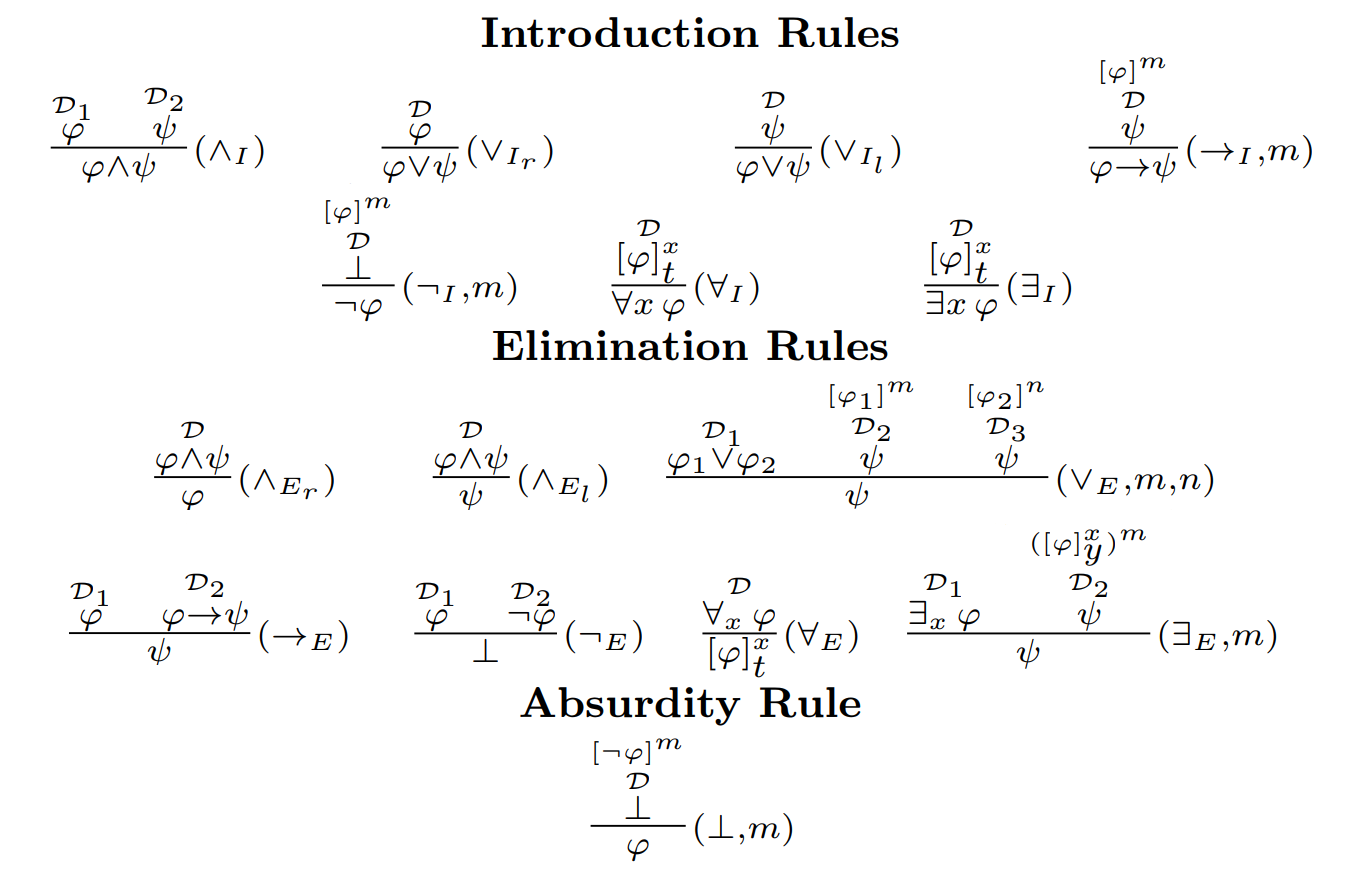
\includegraphics[width=1\linewidth]{resources/rules.png}
    \caption{List of rules for both PL and FOL}
    \label{fig:nd-rules}
\end{figure}

%These proofs can be constructed either bottom-up, from the conclusion to the hypotheses, or top-down, from the hypotheses to the conclusion.  --- talvez não valha a pena dizer isto aqui.

A ND proof is said to be well-formed if and only if it is finite and the inference rules are applied correctly. Moreover, we say that a ND proof proves the consequence \(\Gamma \vdash \phi\) if and only if it is well-formed, the root of the tree is \(\phi\), and every open hypothesis in the tree is contained in \(\Gamma\).
In Fig.~\ref{tab:proof-tree} we have an example of a well-formed ND proof of \( \{\neg (\varphi \lor \psi)\} \vdash \neg \psi \).

\begin{figure}[h]
    \centering
    \[
    \frac{\displaystyle \frac{
    \displaystyle \neg (\varphi \lor \psi)^1 \quad \displaystyle \frac{\psi^2}{(\varphi \lor \psi) \strut} \quad (\lor_{I_l}) \strut}
    {\displaystyle \bot \strut} \quad (\displaystyle \neg_E)\strut} {\displaystyle \neg \psi \strut} \quad (\neg_I, 2)
    \]
    \caption{ND tree proving \( \{\neg (\varphi \lor \psi)\} \vdash \neg \psi \).}
    \label{tab:proof-tree}
\end{figure}
%\begin{definition}[Well-Formed Tree Proof]
%A tree proof is well-formed if and only if it is finite and applies the inference rules correctly.
%\end{definition}
%
%\begin{definition}[Consequence Proven by a Proof]
%Given a tree proof and a problem \(\Gamma \vdash \phi\), we say that the tree solves the problem if and only if it is well-formed and the following conditions both hold:
%\begin{enumerate}
%    \item The root of the tree is \(\phi\).
%    \item Every open hypothesis in the tree is contained in \(\Gamma\).
%\end{enumerate}
%\end{definition}